\section{为什么强化学习对偏差敏感}
\label{sec:diagnosis}

要理解为什么强化学习（RL）对TIM如此敏感，有助于我们理解强化学习与监督微调（SFT）之间的差异。正如我们之前所指出的，即使在训练数据完全由另一个模型离线生成且没有任何重要性采样修正的情况下，SFT仍然保持稳定~\citep{distillation, deepseek_r1}。换句话说，SFT对过时性或内核选择完全不敏感。

至关重要的是，当优势值为 $+1/0$ 时（即奖励未进行中心化或规范化），且训练完全离线（即采样器从未更新），策略梯度在具有二元奖励的任务上退化为 SFT。\footnote{在实际应用中，优势值几乎总是包含负值（例如，由于组中心化 \citep{grpo}），即使训练允许一定程度的延迟，也从不是完全离线的。} 因此，我们可以认为 \textbf{奖励模式} 和 \textbf{延迟性} 是 SFT 与 RL 之间的两个关键差异。\footnote{注意，将奖励平移一个常数不会改变同策略下的期望梯度，而组中心化仅对一组 $G$  回合的奖励进行缩放，缩放因子为 $1 - 1/G$ —— 中心化奖励的原因是它能降低梯度方差 \citep{greensmith, dr_grpo}。  
然而，在异策略情况下这不成立：使用 $+1/0$  的 SFT 收敛到极大似然估计量 \citep{bishop}，而使用 $0/-1$  奖励的 SFT 是退化的：损失会无界增长，可能导致模型坍塌 \citep{finetuning_dynamics}。} 
我们想要确定这两种机制中，哪一种会导致对TIM的敏感性增加。

我们通过一个简单的训练设置来测试这一点，该设置包含有意的策略不匹配。我们对 Qwen3-1.7B \citep{qwen3} 在 Countdown \citep{stream_of_search} 上进行训练，并人为地将采样器的权重与训练器的权重相比进行微小扰动，以创建受控的 TIM。我们在 \Cref{sec:results} 中进一步说明了该设置的理由，并测试了更现实的 TIM 来源。



\begin{figure}[H]
    \centering
    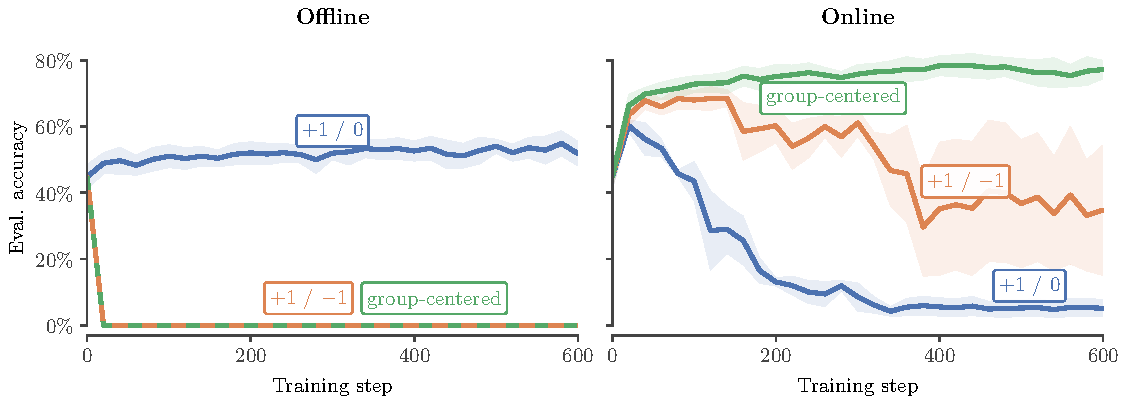
\includegraphics[width=0.9\linewidth]{plots/2b_online_vs_offline.pdf}
    \caption{Qwen3-1.7B 在 Countdown 上三种奖励模式下的离线与在线训练对比。离线训练仅在 $+1/0$ 奖励下稳定，而在线训练在 TIM 模式下于 $+1/0$ 奖励时最不稳定。}
    \label{fig:2b_online_vs_offline}
\end{figure}

\Cref{fig:2b_online_vs_offline} 表明，在此设置下，离线训练仅在 $+1/0$（非负）奖励下稳定，而在线训练则相反——组中心奖励 \citep{grpo}，即组内混合正负值的奖励，是最稳定的，而 $+1/0$ 奖励——对离线训练最稳定——对在线训练却是最不稳定的。因此，我们假设存在两种分离的机制：一种导致离线训练中使用 \textit{负} 奖励时不稳定，另一种则导致在线训练中使用 \textit{正} 奖励时不稳定。

本文的主要关注点是在线强化学习，因此我们不再深入探讨离线训练中负奖励带来的不稳定性。\Citet{finetuning_dynamics} 认为这种不稳定性背后的主要机制在于负奖励的无界性与分布锐化相结合。对数概率从下方无界，因此在带有负奖励的离线训练过程中，它们可能发散至 $-\infty$。这种现象在在线训练中并不存在，因为在在线训练中仅会采样高概率的 token。  
这种不对称性已有充分记录：仅基于正例进行训练（即蒸馏或拒绝微调）即使在离线情况下也完全稳定 \citep{distillation, deepseek_r1}，而负梯度则可能降低正确响应的概率 \citep{nthr}——尽管是同策略的，它们仍携带了有用的学习信号 \citep{negative_reinforcement}。

在在线训练中，我们观察到的行为与离线训练相反——仅使用正向奖励的设置是\emph{最不稳定}的。因此我们假设，这种不稳定性必须源于训练过程的在线特性。
需要注意的是，在TIM下使用$+1/0$奖励进行在线训练本身也是一种蒸馏：训练器被拟合到采样器的成功轨迹上，而采样器是自身的一个有偏副本，其权重在每一步后都从训练器更新。与离线蒸馏唯一的不同在于教师会随着学生移动，因此不稳定性就来源于此。